\section{Desarrollo}
Comenzando con el informe, se conecta el integrado de doble gate, BF966, en configuracion cascode (source común, gate común). El diagrama del circuito utilizado puede verse en la figura \ref{im:circuito}.

\begin{figure}[ht]
	\centering
	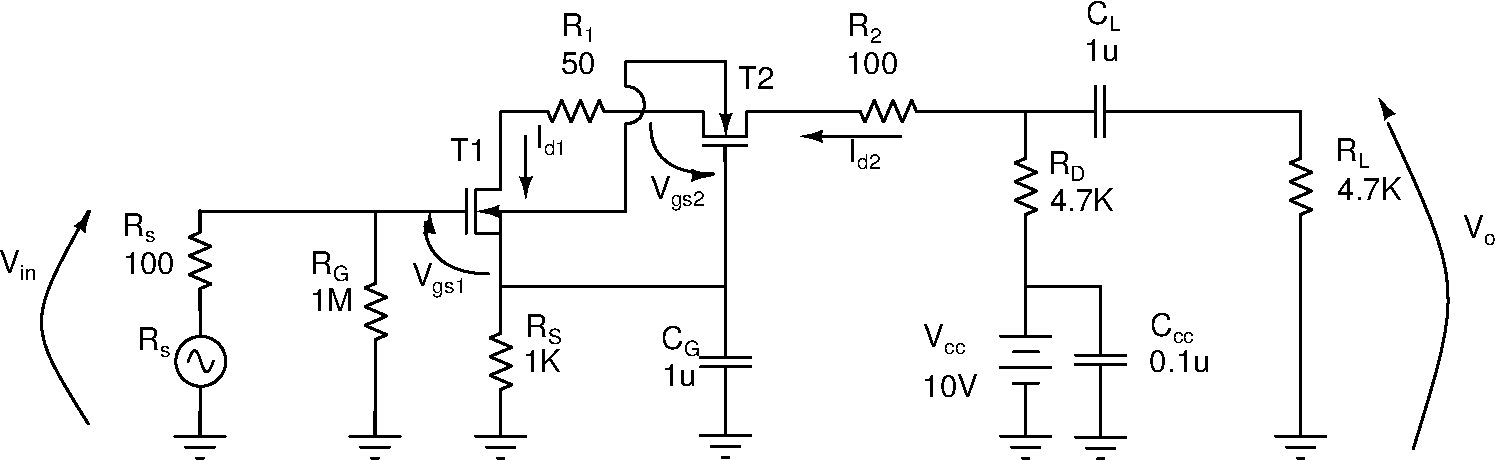
\includegraphics[scale=0.5]{../img/circuitoTL3.pdf}
	\caption{Conexión del circuito a analizar}
	\label{im:circuito}
\end{figure}

Para simplificar el analisis, se admiten por despreciable los parametros $\lambda = 0$ y $\gamma = 0$. De esta forma, no habrá variación de los $V_T$ de cada uno a causa del cortocircuito de los substratos. Viendo la hoja de datos del circuito, se extrajeron los siguientes valores de capacitancias parasitas, que pueden verse en la tabla \ref{ta:capacitanciasParasitas}.

\begin{table}[ht]
\begin{center}
\begin{tabular}{|c|c|c|c|}
\hline 
$C_{issg1}$ & $C_{issg2}$ & $C_{rss}$ & $C_{oss}$ \\ 
\hline 
$2.2\pF$ & $1.1\pF$ & $25\pF$ & $0.8\pF$ \\ 
\hline 
\end{tabular}
\end{center} 
\caption{Valores de capacitancias parasitas del integrado BF966}
\label{ta:capacitanciasParasitas}
\end{table}

El modelo simplificado de la estructura interna del integrado puede verse en la figura \ref{im:modeloIntegrado}.

\begin{figure}[ht]
	\centering 
	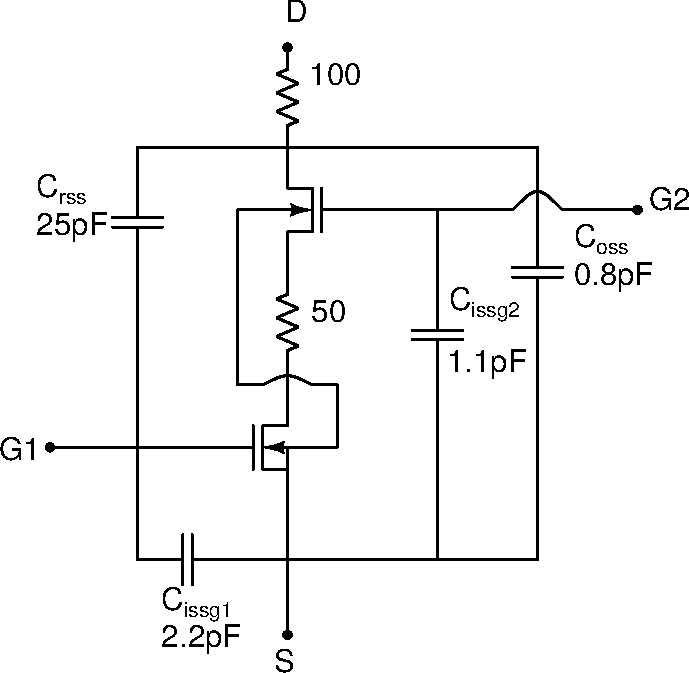
\includegraphics[scale=0.7]{../img/integrados.pdf}
	\caption{Modelo del circuito integrado}
	\label{im:modeloIntegrado}
\end{figure}

Los parametros característicos de ambos transisores pueden verse en la tabla \ref{ta:parametrosTransistor}.

\begin{table}[ht]
\begin{center}
\begin{tabular}{|c|c|c|c|}
\hline 
 & kp & $\VT$ & $\frac{W}{L}$ \\ 
\hline 
T1 & $15\frac{\mA}{\V^2}$ & $-1\V$ & $1$ \\ 
\hline
T2 &  $200\frac{\mA}{\V^2}$  & $-1\V$ & $1$\\
\hline
\end{tabular} 
\end{center}
\end{table}

Se procederá a analizar en primera instancia los valores del reposo del circuito de la figura \ref{im:circuito}. Luego se analizará la amplficación en frecuencias, para finalmente determinar la respuesta de este en bajas y altas frecuencias. Todo esto se hará primero de forma teórica, para luego ser contrastada mediante simulación y por medio de mediciones.